\documentclass{article}\usepackage[]{graphicx}\usepackage[]{color}

\usepackage{alltt}
\usepackage{float}
\usepackage{graphicx}
\usepackage{tabularx}
\usepackage{siunitx}
\usepackage{amssymb} % for math symbols
\usepackage{amsmath} % for aligning equations
\usepackage{textcomp}
\usepackage{mdframed}
\usepackage{natbib}
\usepackage[small]{caption}
\setlength{\captionmargin}{30pt}
\setlength{\abovecaptionskip}{0pt}
\setlength{\belowcaptionskip}{10pt}
\topmargin -1.5cm        
\oddsidemargin -0.04cm   
\evensidemargin -0.04cm
\textwidth 16.59cm
\textheight 21.94cm 
%\pagestyle{empty} %comment if want page numbers
\parskip 7.2pt
\renewcommand{\baselinestretch}{1.5}
\parindent 0pt
%\usepackage{lineno}
%\linenumbers

%% R Script

\title{Evolution constrains tree phenology in experimental settings - Outline}

\begin{document}

\maketitle

\noindent Authors:\\
The Wolkovich Lab in 2019 $^{1,2,3,4}$
\vspace{2ex}\\
\emph{Author affiliations:}\\
$^{1}$Forest \& Conservation Sciences, Faculty of Forestry, University of British Columbia, 2424 Main Mall, Vancouver, BC V6T 1Z4;\\
$^{2}$Arnold Arboretum of Harvard University, 1300 Centre Street, Boston, Massachusetts, USA;\\
$^{3}$Organismic \& Evolutionary Biology, Harvard University, 26 Oxford Street, Cambridge, Massachusetts, USA;\\
$^{4}$Edificio Ciencias, Campus Universitario 28805 Alcalá de Henares, Madrid, Spain\\
 

\vspace{2ex}
$^*$Corresponding author: ignacio.moralesc@uah.es\\
\renewcommand{\thetable}{\arabic{table}}
\renewcommand{\thefigure}{\arabic{figure}}
\renewcommand{\labelitemi}{$-$}
\setkeys{Gin}{width=0.8\textwidth}

%%%%%%%%%%%%%%%%%%%%%%%%%%%%%%%%%%%%%%%%%%%%%%%
%%%%%%%%%%%%%%%%%%%%%%%%%%%%%%%%%%%%%%%%%%%%%%%
\clearpage
\section*{Rationale \& Significance}

Previous work has looked at the phylogenetic conservatism of phylogenies across plant species, finding that, first flowering is significantly conserved \citep{davies2013phylogenetic} and, when using OU models so are shifts in first flowering \citep{rafferty2017global}.\\ 

Nevertheless, previous work on the phylogenetic conservatism of phenology has still not addressed:\\
- Are phenological responses in lab experiments conserved as well? In \cite{joly2019importance} the authors check this but with a focus in intraspecific variations\\
- How the sensitivities to different environmental cues are conserved?\\
- Are the responses to cues more strongly conserved than others?\\
- How does accounting for phylogeny affects model estimations of cue sensitivity?\\

The potential interest of findings in this direction stem from:\\
- better predictions of phenology (or need to account for it in models)\\
- better understand the mechanistic basis of plant responses to climate\\
- better design the next generation of experiments \\


\section*{Abstract}
\begin{enumerate}
\item How plants respond to environmental cues--i.e. temperature, daylight--may determine their resilience or vulnerability to ongoing climate change. 
\item Phenology provides a good description of plant responses to to the environment. 
\item Phenology has been regarded to as a rather plastic trait, thus with a lot of variation both intra- and inter-specifically.
\item Variation in phenology could have randomly accummulated across species (and then phenology would be an evolutionary labile trait), or be structured in the phylogeny so that closely related species resemble more each other in their phenological responses (conserved trait).
\item Whether or not phenology is conserved has implications for the need to account for phylogenetic autocorrelation in cross-species analyses.
\item More interestingly, given that phylogeny can act as a proxy for other (unaccounted) traits that may be linked to phenology, including it in models could lead to more accurate predictions.
\item Here we use Bayesian hierarchical models and the most complete dataset on tree species phenological responses measured in experimental conditions to: (a) test if tree species responses to cues are conserved phylogenetically, (b) compare the phylogenetic signal in the responses to different cues and, (c) test the abiltiy of phylogenetically informed models to improve predictive accuracy of phenology.
\item Results show non-random phylogenetic structuring of phenological responses, highly variable across cues.  
\item Taken together, our results suggest that phylogeny should be incorporated into studies modelling multi-species phenological responses, as such responses have been constrained through evolution and thus are not independent.  
\end{enumerate}

% not yet satisfied about the pitch - this is already said in Davies et al. 2013 
% should we emphasize the fact that we are using experimental/lab data? What are the gains with respect data from the field?

% we need an angle of at least some novelty



\section*{Introduction}
\begin{enumerate}
\item Phenology is a critical trait to studying biological responses to climate change.
\item Forecasts of phenological responses to environmental change are very important (e.g. agriculture, pest management, etc.) but they are not successful, partly due to data limitations: many species lack data and even those with data may have incomplete time series for all relevant phenophases. Could we impute missing data using phylogeny as a proxy? 
\item Phenology has been shown to be phylogenetically conserved, but studies to date are limited by:
\begin{enumerate}
\item focused on flowering (and leafout some) times and shifts in them (but see \cite{joly2019importance})
\item studied trait correlation \citep{bolmgren2008time}
\item studied evolutionary models best fitting the data \citep{rafferty2017global}
\item measured shifts based on field observation data for both climate and phenology (when slopes are available, they represent the response to one cue only: forcing)
\end{enumerate}
\item Few examples in the literature have tested for phylogenetic signal of phenological responses using growth chamber data (e.g. \cite{joly2019importance}, and yet such a source of data could have advantages such as:
\begin{enumerate}
\item it makes possible to examine responses to more than one cue and thus not restrict analyses to responses to forcing.
\item it is possible to compare responses to cues (are some more conserved than others?) 
\item they may allow testing whether phylogeny can improve models of phenology as a response to a cue
\end{enumerate}
\end{enumerate}



\section*{Methods}
\subsection*{Phenological and Phylogenetic Data}
\begin{enumerate}
\item Description of the OSPREE database (where it comes from, number of species, studies, etc.) and how we prune it to retain the final list of 62 species. 
\item Two phylogenetic hypotheses have been considered to build a tree containing the species in OSPREE. First the vascular plant megatree by Zanne et al. (2014);Nature and, second the megatree by Smith \& Brown (2019);AJB.
\end{enumerate}

\subsection*{Provenance-climate Data}
\begin{enumerate}
\item Should we test/analyze provenace or climate-effects? If so, we would need to 
\end{enumerate}

\subsection*{Data Analysis}
\begin{enumerate}
\item We used a Bayesian hierarchical model approach to estimate the number of days until budburst is reached as a function of forcing, chilling and photoperiod. 

\item The Bayesian hierarchical model was fit using the brms package \citep{brms}, in R \citep{R}, version 3.5.1, and followed the notation: 

\item Copy model specifications below (TBD).

\item Specify model evaluation and metrics of accuracy (Rhat, Rsq, more?)

\item To test the ability of phylogeny to improve models/predictions of budburst we: (describe procedure)


\subsection*{The Bayesian Phylogenetic hierarchical model}

\item Explain how the model is fit, and how the $H^{2}$ metric is analogous to lambda in PGLS.


\end{enumerate}


\section*{Results}
\subsection*{Phylogenetic signal in phenological responses}
\begin{enumerate}
\item Phenological responses to the three studied cues are overall phylogenetically conserved but estimates of phylogenetic signal differ across species subsets.
\item When all species are considered, responses to forcing are more conserved ($H^{2}$ = 0.73) than responses to chilling ($H^{2}$ = 0.47) or to photoperiod ($H^{2}$ = 0.55) (see Figure \ref{fig:phylosig_spp}).  
\item When species belonging to the same genera (usually showing large polytomies in the phylogeny) are grouped into species complexes (for which data on cross-treatments are more complete), responses to forcing ($H^{2}$ = 0.37) and photoperiod ($H^{2}$ = 0.68) are conserved but responses to chilling ($H^{2}$ = 0.18) are not Figure \ref{fig:phylosig_complex}).  
\item The marked differences in the responses to each cue are buffered when only angiosperm species are considered, with all responses being mildly conserved: forcing ($H^{2}$ = 0.33), chilling ($H^{2}$ = 0.37) and photoperiod ($H^{2}$ = 0.40). This suggests gymnosperms, even few species can have a major  effect in apparent differences across cues (Figure \ref{fig:phylosig_angiosperm}). 
\item The correlations among responses to the cues are positive but only markedly high between photoperiod and chilling (Figure \ref{fig:sensicorrs}).
\end{enumerate}


\subsection*{Budburst models, phylogenetic and non-phylogenetic}
\begin{enumerate}
\item Insert table here summarizing changes in coefficients and Rsq with/without phylogeny
\end{enumerate}




\section*{Discussion}
\begin{enumerate}
\item To be fleshed out.
  

\end{enumerate}
  
  



\bibliography{phylorefs}
\bibliographystyle{amnat}

\section*{Tables and Figures} 

\begin{figure} [H]
  \begin{center}
  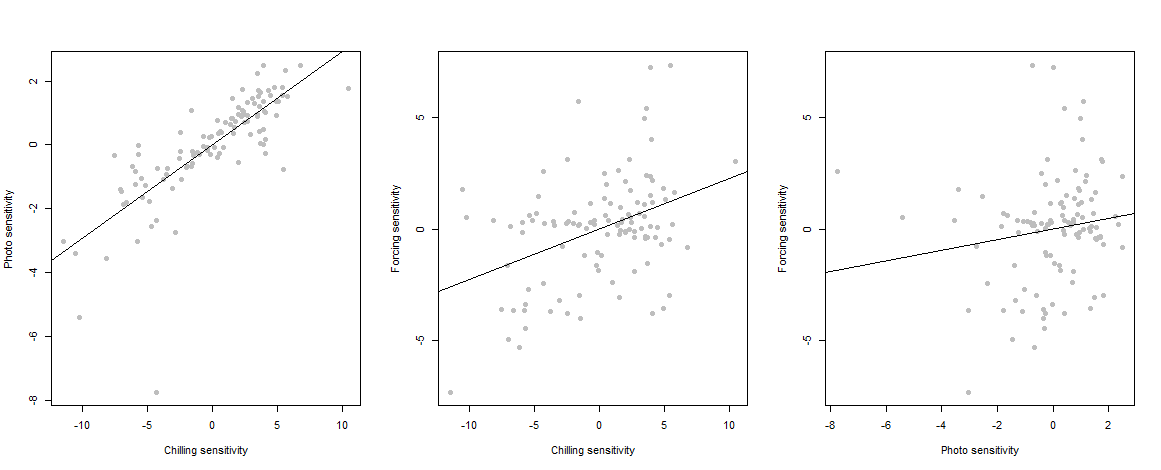
\includegraphics[width=14cm]{..//..//analyses/phylogeny/figures/Correlations_sensitivities.png}
  \caption{Scatterplots showing correlations between the sensitivities of the species in OSPREE to chilling and photoperiod (A), chilling and forcing (B), and forcing and photoperiod (C). Sensitivities are  correlated overall, but more so between chilling and photoperiod.}
  \label{fig:sensicorrs}
  \end{center}
\end{figure}

  
\begin{figure} [H]
  \begin{center}
  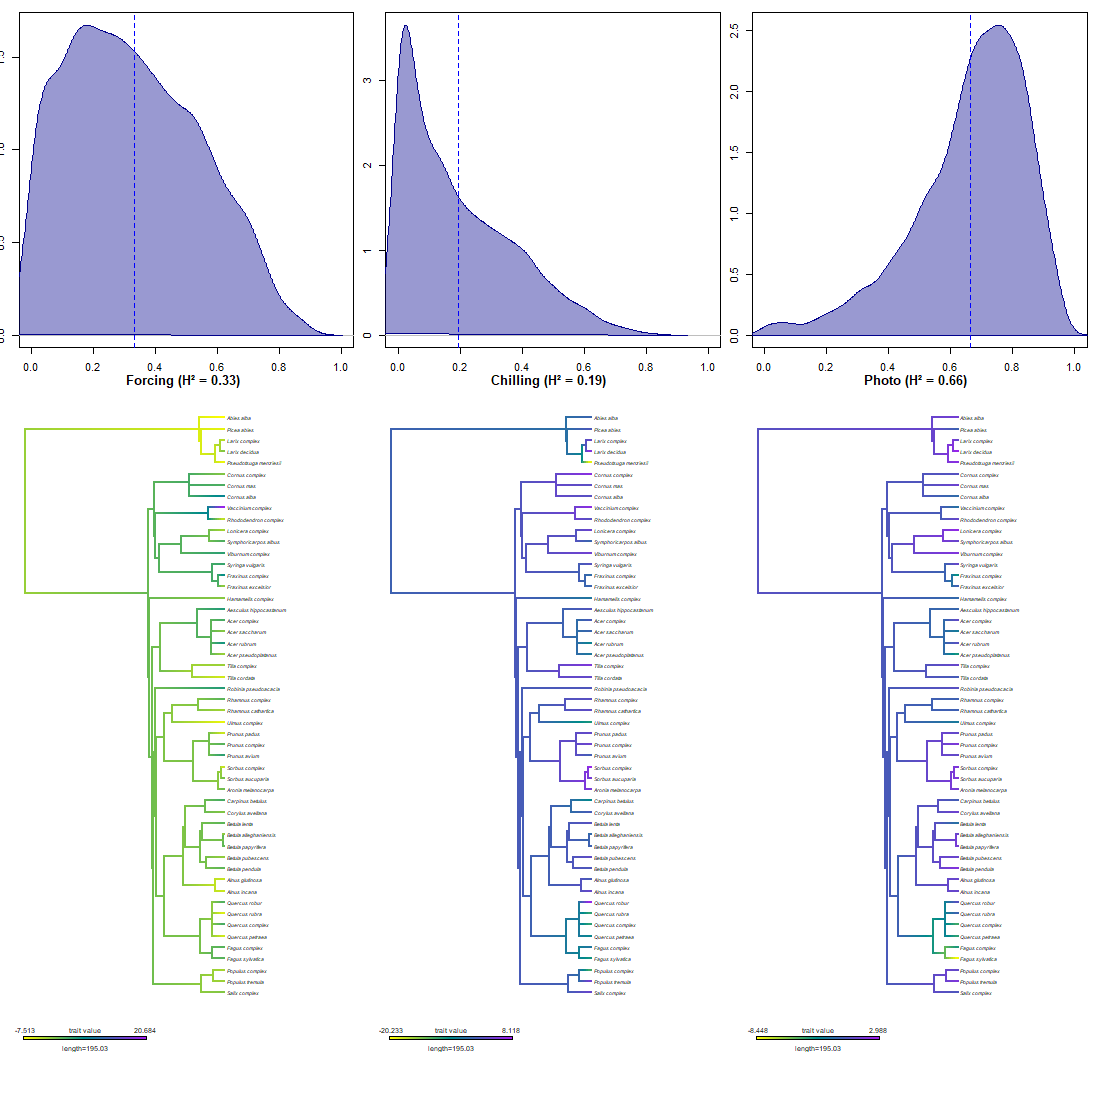
\includegraphics[width=14cm]{..//..//analyses/phylogeny/figures/Sensitivities_phylosig.png}
  \caption{Phylogenetic signal results for the sensitivities of each species complex (species grouped by genera) to the forcing (A), chilling (B) and photoperiod (C) cues.}
  \label{fig:phylosig_complex}
\end{center}
\end{figure}

\begin{figure} [H]
  \begin{center}
  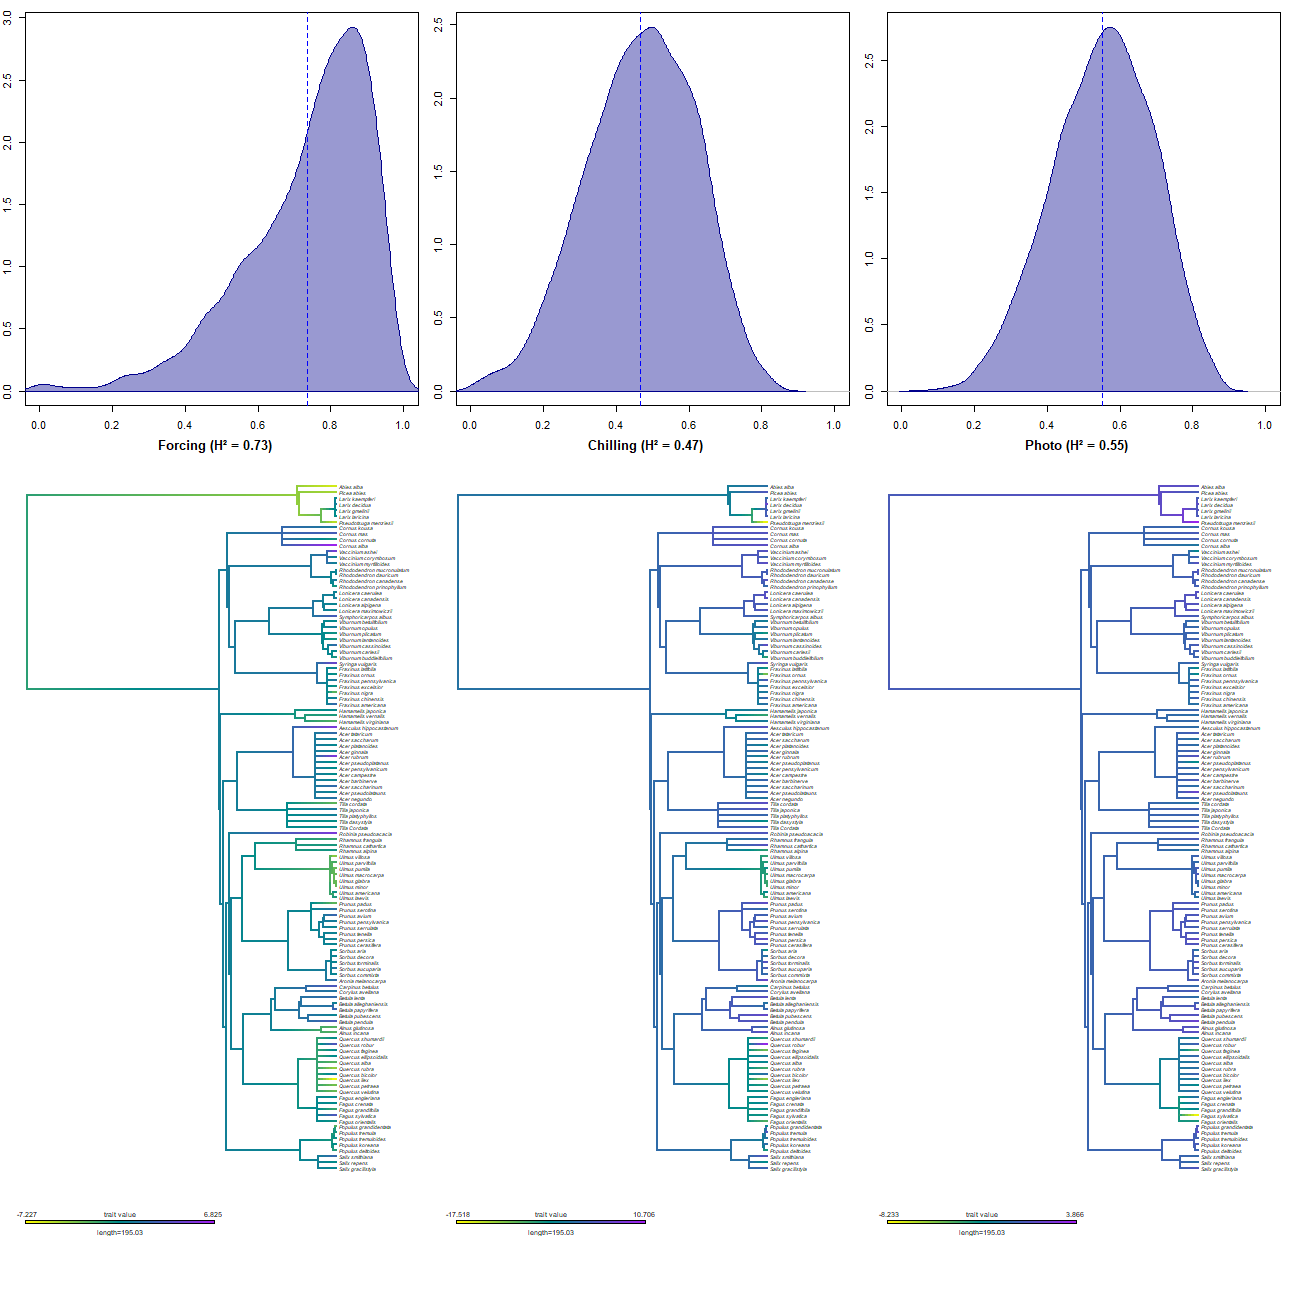
\includegraphics[width=14cm]{..//..//analyses/phylogeny/figures/Sensitivities_phylosig_spslev.png}
  \caption{Phylogenetic signal results for the sensitivities of each species (ungrouped) to the forcing (A), chilling (B) and photoperiod (C) cues.}
  \label{fig:phylosig_spp}
  \end{center}
  \end{figure}

\begin{figure} [H]
  \begin{center}
  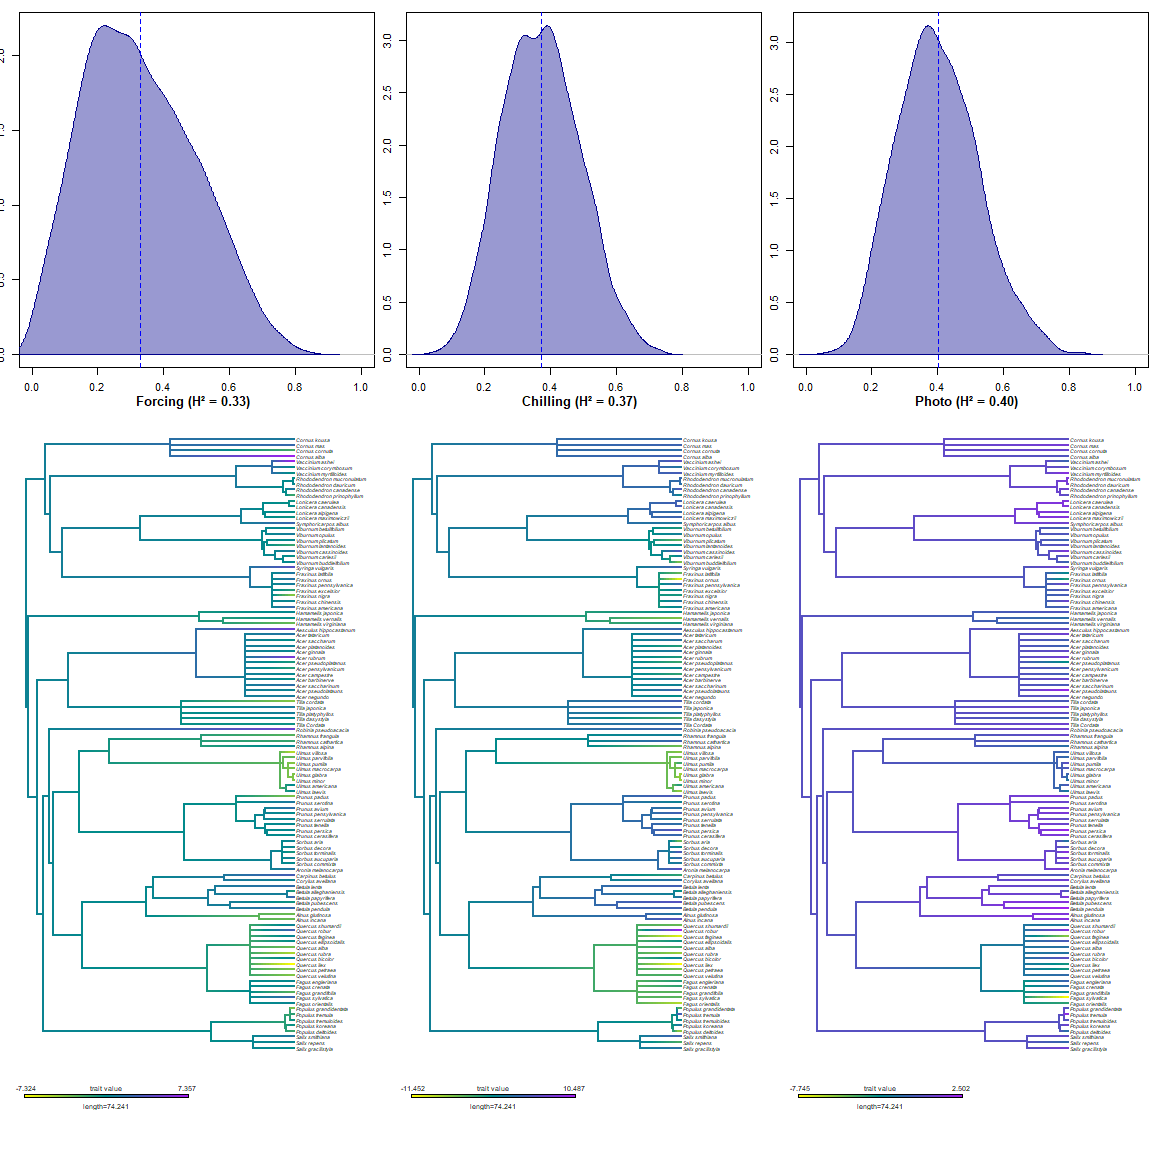
\includegraphics[width=14cm]{..//..//analyses/phylogeny/figures/Sensitivities_phylosig_spslev_angiosperms.png}
  \caption{Phylogenetic signal results for the sensitivities of each species (excluding gymnosperms) to the forcing (A), chilling (B) and photoperiod (C) cues.}
  \label{fig:phylosig_angiosperm}
  \end{center}
\end{figure}

\end{document}
